\documentclass[10pt, aspectratio=169]{beamer}
\usefonttheme{professionalfonts}

\mode<presentation>
{
  \usetheme{Berkeley}
  \usecolortheme{beaver}
  \usefonttheme{default}
  \setbeamertemplate{navigation symbols}{}
  \setbeamertemplate{caption}[numbered]
} 

\setbeamertemplate{footline}{%
  \leavevmode%
  \hbox{%
    \begin{beamercolorbox}[wd=.85\paperwidth,ht=2.5ex,dp=1ex,left]{author in head/foot}%
      \usebeamerfont{author in head/foot}Maxx Seminario, Electronic Circuits, Spring 2026%
    \end{beamercolorbox}%
    \begin{beamercolorbox}[wd=.15\paperwidth,ht=2.5ex,dp=1ex,right]{date in head/foot}%
      \hspace*{0.5em}\insertframenumber{} / \inserttotalframenumber\hspace*{0.5em}%
    \end{beamercolorbox}%
  }%
  \vskip0pt%
}

\usepackage[english]{babel}
\usepackage[utf8x]{inputenc}
\usepackage{tikz}
\usetikzlibrary{shapes.geometric}
\usepackage{pgfplots}
\usepackage{array}
\usepackage{makecell}
\usepackage{verbatim}
\usepackage{graphicx}
\usepackage{subcaption}
\usepackage{amsfonts}
\usepackage{amsmath}
\usepackage{bm}
\usepackage{epstopdf}
\usepackage{circuitikz}
\usepackage{caption}
\usepackage{multirow}
\captionsetup{compatibility=false}
\usepackage[absolute,overlay]{textpos}
\usetikzlibrary{calc}
\usetikzlibrary{pgfplots.fillbetween, backgrounds}
\usetikzlibrary{positioning}
\usetikzlibrary{pgfplots.groupplots}
\usetikzlibrary{plotmarks}
\usetikzlibrary{calc}

\pgfplotsset{compat=1.16}

\title{MOSFET DC Analysis and Biasing}
\subtitle{Unit 5: Field-Effect Transistors}
\author{Maxx Seminario}
\institute{University of Nebraska-Lincoln}
\date{Spring 2026}

\begin{document}

\begin{frame}
  \titlepage
\end{frame}

% Slide 2: Lecture Overview
\begin{frame}{Lecture Overview}
\begin{columns}
\begin{column}{0.45\textwidth}
\textbf{Review from Last Lecture}
\begin{itemize}
\item MOSFET device structure
\item Operating regions (cutoff, linear, saturation)
\item I-V characteristics
\item Field effect and channel modulation
\end{itemize}
\end{column}


\begin{column}{0.45\textwidth}
\textbf{Learning Objectives}
\begin{itemize}
\item Analyze MOSFET DC circuits
\item Determine Q-point for different bias configurations
\item Design bias circuits for specified operating points
\end{itemize}
\end{column}
\end{columns}
\end{frame}

% Slide 3: DC Operating Point (Q-Point)
\begin{frame}{DC Operating Point (Q-Point)}
\begin{columns}
\begin{column}{0.5\textwidth}
\textbf{What is the Q-Point?}
\begin{itemize}
\item Quiescent operating point
\item DC voltages and currents with no signal
\item Determines transistor operating region
\end{itemize}

\textbf{Q-Point Parameters:}
\begin{itemize}
\item $V_{GS}$: Gate-source voltage
\item $V_{DS}$: Drain-source voltage
\item $I_{DS}$: Drain-source current
\end{itemize}

% \vspace{0.3cm}

\textbf{Design Goals:}
\begin{itemize}
\item Ensure proper operating region
\item Maximize voltage swing
\item Minimize power consumption
\end{itemize}
\end{column}

\begin{column}{0.5\textwidth}
\textbf{Q-Point on I-V Characteristics}

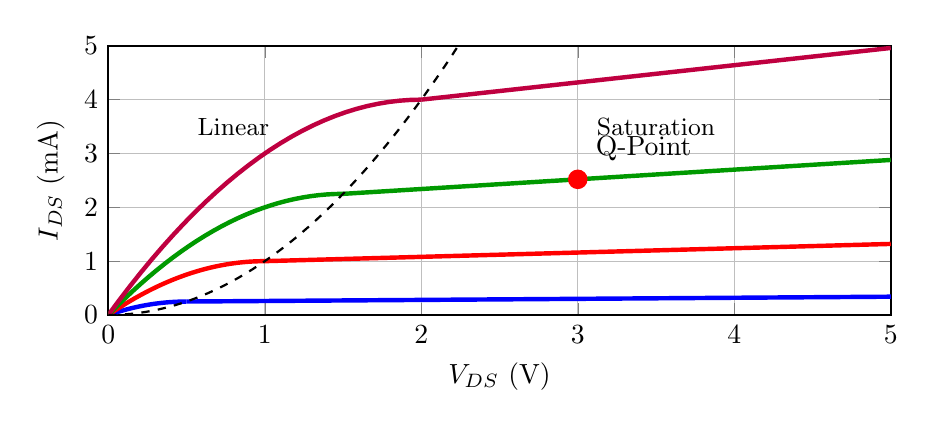
\begin{tikzpicture}
\begin{axis}[
    width=0.95\textwidth,
    height=5cm,
    xlabel={$V_{DS}$ (V)},
    ylabel={$I_{DS}$ (mA)},
    xmin=0, xmax=5,
    ymin=0, ymax=5,
    xtick={0, 1, 2, 3, 4, 5},
    ytick={0, 1, 2, 3, 4, 5},
    grid=major,
    thick,
]

% VGS = 1.0V (V_OV = 0.5V)
\addplot[blue, ultra thick, domain=0:0.5, samples=30] {x - x^2};
\addplot[blue, ultra thick, domain=0.5:5, samples=30] {0.25*(1+0.08*(x-0.5))};

% VGS = 1.5V (V_OV = 1.0V)
\addplot[red, ultra thick, domain=0:1.0, samples=30] {2*x - x^2};
\addplot[red, ultra thick, domain=1.0:5, samples=30] {1.0*(1+0.08*(x-1.0))};

% VGS = 2.0V (V_OV = 1.5V)
\addplot[green!60!black, ultra thick, domain=0:1.5, samples=30] {3*x - x^2};
\addplot[green!60!black, ultra thick, domain=1.5:5, samples=30] {2.25*(1+0.08*(x-1.5))};

% VGS = 2.5V (V_OV = 2.0V)
\addplot[purple, ultra thick, domain=0:2.0, samples=30] {4*x - x^2};
\addplot[purple, ultra thick, domain=2.0:5, samples=30] {4.0*(1+0.08*(x-2.0))};

% Saturation boundary (parabola)
\addplot[black, dashed, thick, domain=0:2.236, samples=50] {x^2};

% Q-point (at VGS=2.0V, VDS=3V)
\node[circle, fill=red, inner sep=2.5pt, label=above right:{Q-Point}] at (axis cs:3,2.52) {};

% Region labels
\node[font=\small] at (axis cs:0.8,3.5) {Linear};
\node[font=\small] at (axis cs:3.5,3.5) {Saturation};
\end{axis}
\end{tikzpicture}

\vspace{-0.1cm}

\begin{block}{Key Concept}
The Q-point sets the DC bias, determining where the transistor operates and its 'behavior / character'.
\end{block}
\end{column}
\end{columns}
\end{frame}

% Slide 4: DC Analysis Procedure
\begin{frame}{DC Analysis General Procedure}
\begin{enumerate}
\item \textbf{Assume an operating region} 

\vspace{0.3cm}
\item \textbf{Apply KVL and KCL} to the circuit
   \begin{itemize}
   \item Use DC voltage sources only (capacitors open, inductors short)
   \item Write node and loop equations
   \end{itemize}

\vspace{0.3cm}
\item \textbf{Apply MOSFET equations} for the assumed region
   \begin{itemize}
   \item Saturation: $I_D = \frac{1}{2} \mu_n C_{ox} \frac{W}{L} (V_{GS} - V_{th})^2$
   \item Linear: $I_D = \mu_n C_{ox} \frac{W}{L} \left[ (V_{GS} - V_{th}) V_{DS} - \frac{V_{DS}^2}{2} \right]$
   \item Cutoff: $I_D = 0$
   \end{itemize}

\vspace{0.3cm}
\item \textbf{Solve for unknowns}: $V_{GS}$, $V_{DS}$, $I_D$

\vspace{0.3cm}
\item \textbf{Verify the assumption from step 1}
   \begin{itemize}
   \item Saturation: Check $V_{DS} \geq V_{GS} - V_{th}$ and $V_{GS} > V_{th}$
   \item Linear: Check $V_{DS} < V_{GS} - V_{th}$ and $V_{GS} > V_{th}$
   \item If violated, re-analyze with correct region
   \end{itemize}
\end{enumerate}
\end{frame}

% Slide 5: Fixed Gate Bias Configuration
\begin{frame}{Fixed Gate Bias Configuration}
\begin{columns}
\begin{column}{0.35\textwidth}

\textbf{Circuit Schematic}

\begin{circuitikz}[scale=0.75, transform shape]
% VDD
\draw (0,5) to[short, o-] (0,4.5) node[above] at (0,5) {$V_{DD}$};
% RD
\draw (0,4.5) to[R, l=$R_D$] (0,2.5);
% MOSFET
\draw (0,2.5) node[nmos, arrowmos, anchor=drain] (M1) {};
\draw (M1.source) to[short] (0,0) node[ground] {};
% Gate bias
\draw (-2.5,1.7) to[short, o-] (-2.5,1.75) node[left] {$V_{GG}$};
\draw (-2.5,1.7) to[R, l=$R_G$] (-1,1.7);
\draw (-1,1.7) to[short] (M1.gate);
% Output
\draw (0,2.5) to[short, -o] (1,2.5) node[right] {$v_D$};
\end{circuitikz}


\end{column}

\begin{column}{0.6\textwidth}
\textbf{DC Analysis:}

Given: $V_{DD}$, $V_{GG}$, $R_D$, $R_G$, $V_{th}$, $k_n = \frac{1}{2} \mu_n C_{ox} \frac{W}{L}$

\vspace{0.3cm}

\textbf{Step 1:} Gate-source voltage (assume $I_G = 0$)
\[
V_{GS} = V_G - V_S = V_{GG}
\]

\textbf{Step 2:} Drain current (assuming saturation)
\[
I_D = k_n (V_{GS} - V_{th})^2 = k_n (V_{GG} - V_{th})^2
\]

\textbf{Step 3:} Drain voltage (KVL)
\[
V_{DS} = V_D - V_S = V_{DD} - I_D R_D
\]

\textbf{Step 7:} Verify saturation (our previous assumption)
\[
V_{DS} \geq V_{GS} - V_{th} 
\]
\end{column}
\end{columns}
\end{frame}

% Slide 7: Voltage Divider Bias
\begin{frame}{Voltage Divider Bias Configuration}
\begin{columns}
\begin{column}{0.45\textwidth}

\vspace{-0.3cm}

\textbf{Circuit Diagram}

\begin{circuitikz}[scale=0.65, transform shape]
% VDD
\draw (0,6) to[short, o-] (0,5.5) node[above] at (0,6) {$V_{DD}$};
% RD
\draw (0,5.5) to[R, l=$R_D$] (0,3.5);
% MOSFET
\draw (0,3.5) node[nmos, arrowmos, anchor=drain] (M1) {};
% RS
\draw (M1.source) to[R, l=$R_S$] (0,0) node[ground] {};
% Voltage divider
\draw (-3,5.5) to[short] (-3,5.5) node[above] {$V_{DD}$};
\draw (-3,5.5) to[R, l=$R_1$] (-3,2.75);
\draw (-3,2.75) to[R, l=$R_2$] (-3,0) node[ground] {};
\draw (-3,2.75) to[short, *-] (M1.gate);
% Output
\draw (0,3.5) to[short, -o] (1,3.5) node[right] {$v_D$};
\end{circuitikz}

\begin{itemize}
\item Most common biasing method
\item Best stability
\item Independent of device parameters if designed properly
\end{itemize}
\end{column}

\begin{column}{0.55\textwidth}
\textbf{DC Analysis:}

\textbf{Gate and Source voltages} 
\[
\begin{aligned}
V_G &= V_{DD}\frac{R_2}{R_1+R_2}, \qquad
V_S &= I_D R_S
\end{aligned}
\]

\vspace{-0.8cm}

\[
V_{GS} = V_G - V_S = V_{DD} \frac{R_2}{R_1 + R_2} - I_D R_S
\]

\textbf{Drain current (assume saturation)}
\[
I_D = k_n (V_{GS} - V_{th})^2
\]

\vspace{-0.1cm}

Substitute and solve quadratic for $I_D$.

\textbf{Drain-Source voltage}
\[
V_D = V_{DD} - I_D R_D, 
\]

\vspace{-0.8cm}

\[
V_{DS} = V_D - V_S = V_{DD} - I_D (R_D + R_S)
\]


\end{column}
\end{columns}
\end{frame}

% Slide 9: Design Considerations
\begin{frame}{Design Considerations for DC Biasing}
\begin{columns}[T]
\begin{column}{0.5\textwidth}
\textbf{Operating Region}
\begin{itemize}
\item For amplifiers: saturation region
\item Ensure $V_{DS} \geq V_{GS} - V_{th}$
\end{itemize}

\vspace{0.3cm}
\textbf{Voltage Swing}
\begin{itemize}
\item Maximize output voltage range
\item Center Q-point on load line
\item Typical: $V_{DS} \approx \frac{V_{DD}}{2}$
\end{itemize}

\vspace{0.3cm}
\textbf{Power Dissipation}
\begin{itemize}
\item $P_D = V_{DS} \cdot I_D$
\item Consider thermal limits
\item Trade-off with performance
\end{itemize}
\end{column}

\begin{column}{0.5\textwidth}

\vspace{0.3cm}
\textbf{Component Selection}
\begin{itemize}
\item Consider tolerances
\item Power ratings for resistors
\end{itemize}

\vspace{0.3cm}
\textbf{Design Steps}
\begin{enumerate}
\item Choose $I_D$ based on application
\item Set $V_{DS}$ for desired swing
\item Calculate required $V_{GS}$
\item Design bias network
\item Verify operation through simulation 
\end{enumerate}
\end{column}
\end{columns}
\end{frame}

% Slide 10: Example Problem - Voltage Divider Bias
\begin{frame}{Example: Voltage Divider Bias Design}
\begin{columns}[T]
\begin{column}{0.45\textwidth}
\textbf{Given:}
\begin{itemize}
\item $V_{DD} = 12$ V
\item $V_{th} = 1$ V
\item $k_n = 2$ mA/V$^2$
\item Design for: $I_D = 2$ mA, $V_{DS} = 6$ V
\end{itemize}

\textbf{Step 1:} Choose $V_S$ (Artist's choice)
\[
V_S = 2 \text{ V}
\]

\textbf{Step 2:} Calculate $R_S, V_D$ 
\[
R_S = \frac{V_S}{I_D} = \frac{2}{2 \times 10^{-3}} = 1 \text{ k}\Omega
\]

\vspace{-0.55cm}

\[
V_D = V_S + V_{DS} = 2 + 6 = 8 \text{ V}
\]
\end{column}

\begin{column}{0.55\textwidth}
\textbf{Step 3:} Calculate $R_D$
\[
R_D = \frac{V_{DD} - V_D}{I_D} = \frac{12 - 8}{2 \times 10^{-3}} = 2 \text{ k}\Omega
\]

\textbf{Step 4:} Find required $V_{GS}$ (assume saturation)
\[
I_D = k_n (V_{GS} - V_{th})^2
\]
\[
2 = 2 (V_{GS} - 1)^2 
\]
\[
\begin{aligned}
V_{GS} = 2 \text{ V} \quad
V_G = 4 \text{ V}
\end{aligned}
\]

\textbf{Step 6:} Design voltage divider

\[
\frac{R_2}{R_1 + R_2} = \frac{V_G}{V_{DD}} = \frac{4}{12} = \frac{1}{3}
\]
\[
R_2 = 20 \text{ k}\Omega, \quad R_1 = 40 \text{ k}\Omega
\]
\end{column}
\end{columns}
\end{frame}

% TODO: Incude summary slide? May not be needed here.

\end{document}
